% -*- root: ../EstadisticaII.tex -*-
\chapter{Contrastes no paramétricos}
\section{Introducción}
\begin{defn}[Hipótesis no paramétrica]
Hipótesis que no se formula en términos de un número finito de parámetros.\end{defn}

En este capítulo vamos a ver 3 tipos de contrastes (con diferentes test para algunos contrastes)
\begin{enumerate}
\item \textbf{Bondad de ajuste:} A partir de una muestra $X_1,...,X_n \equiv F$ de variables aleatorias independientes idénticamente distribuidas, contrastar:
\begin{itemize}
\item $H_0: F=F_0$ donde $F_0$ es una distribución prefijada.
\item $H_0: F \in \{F_{\theta} : {\theta}\in H\}$, donde H es el espacio paramétrico.
\end{itemize}
\item \textbf{Homogeneidad:} Dados $X_1,...,X_n \equiv F$ y $Y_1,...,Y_n \equiv G$ de variables aleatorias independientes idénticamente distribuidas. Contrastar $H_0: F=G$.
\item \textbf{Independencia:} Dada $(X_1,Y_1),...,(X_n,Y_n) \equiv F$ de variables aleatorias independientes idénticamente distribuidas. Contrastar $H_0: X$ e $Y$ son independientes.
\end{enumerate}


%%%%%%%%%%%%%%%%%%%%%%%%%%%%%%%%%%%%%%%%%%%%%%%%%%%%%%%%%%%%%%%%%%%%%%%%%%%%%%%%%%%%%%%%%%%%%%%%%%

\section{Contrastes de bondad de ajuste}

\subsection{Contraste $\chi^2$ de bondad de ajuste}
Consideramos una distribución totalmente especificada bajo $H_0: X_1,...,X_n \equiv F$ de variables i.i.d.

$H_0: F=F_0$ es la hipótesis nula y queremos ver que F, que es la distribución obtenida con los datos verdaderos (obtenidos empíricamente) es igual a $F_0$ que es la distribución teórica.

Vamos a definir los pasos que tenemos que seguir para comprobar si $H_0$ es cierta:
\begin{enumerate}
\item Se definen k clases $A_1,...,A_k$. En el caso del dado, los valores de cada cara.
\item Se calculan las frecuencias observadas de datos en cada clase.
\subitem \[O_i = \#\{j\tq X_j ∈ A_i\}\]
\[O_i \sim Bin\left(n,p_i = p_{H_0}(A_i)\right) \text{ es una variable aleatoria}\]
\item Se calculan las frecuencias esperadas si $H_0$ fuera cierta:
	\subitem\[\esp{F}_i = \esp{F}_{H_{0}} = np_i \text{ al ser } O_i \text{ una binomial}\]
\item Se comparan $O_i$ con $E_i$ mediante el estadístico de Pearson, para comprobar si lo observado se parece a lo esperado.

\[T = \sum_{i=1}^k \frac{(O_i - E_i)^2}{E_i}\]

\subitem Más adelante justificaremos porqué este estadístico es el utilizado. Además, el estadístico puede calcularse de otra manera:

\[
T = \sum \frac{O_i^2}{E_i} - n
\]
\item Se rechaza $H_0$ en la región crítica $R = \{ T>c\}$, donde $c$ depende del nivel de significación $α$.
\subitem $c$ se obtiene consultando en las tablas para $α = P_{H_0}(T>c)$
\end{enumerate}

Pero se nos presenta el siguiente problema, ¿Cuál es la distribución de $T$ bajo $H_0$?

\begin{theorem}[Estadístico\IS de Pearson]
El estadístico de Pearson es:
\[T = \sum_{i=1}^k \frac{(O_i - E_i)^2}{E_i} = \sum \frac{O_i^2}{E_i} - n\]

Además, bajo $H_0$ su distribución:

\[
T \convs[d] \chi^2_{k-1}
\]
\end{theorem}

\begin{proof}
\textcolor{red}{Para otro momento}
\end{proof}

\begin{example}
Tiramos un dado 100 veces y obtenemos:

\begin{tabular}{|c|c|c|c|c|c|c|}
\hline
Resultados & 1 & 2 & 3 & 4 & 5 & 6 \\
\hline
Frecuencia & 10 & 20 & 20 & 10 & 15 & 25\\
\hline
\end{tabular}

Y consideramos $H_0: p_i=\frac{1}{6} \; \forall i=1,...,6$. Es decir que el dado no está trucado y cada cara tiene la misma probabilidad ($p_i$) de salir.

¿Es cierta la hipótesis, con un nivel de confianza/significación del 95\%?


Las clases son cada uno de los posibles resultados y las frecuencias observadas se encuentran en la tabla.

Vamos a calcular el estadístico $T$ \[T = \sum_{i=1}^6 \frac{O_i^2}{E_i} - n = \frac{6}{100} (\sum O_1^2) - 100 = ... = 11\]

Ahora, consultando las tablas buscamos el valor $\chi^2_{5;0.05} = 11.07 > T = 11$, entonces no estamos en la región crítica, por lo que no podemos rechazar la hipótesis.

Al ser valores muy próximos, observamos que el p-valor\footnote{el menor nivel de confianza para poder rechazar} del contraste tendrá que ser algo mayor que $0.05$.

\end{example}







\subsubsection{Hipótesis nula compuesta}

Vamos a estudiar el siguiente problema. Sea $X_1,...,X_n \overset{}{\sim}{iid}  F$ y una hipótesis compuesta: $H_0: F\in \{ F_{\theta}, \theta\in Ω \subset ℝ^n\}$. Esta hipótesis compuesta puede ser ``los datos se distribuyen normalmente, con media y varianza desconocidas''

Los pasos a seguir son:
\begin{enumerate}
	\item Definir las clases $A_1,...,A_k$
	\item Calcular las frecuencias observadas $O_1,...,O_n$
	\item Estimamos $\theta$ por el método de máxima verosimilitud. Sea $\gor{\theta}$ el e.m.v.
	\subitem Pero para calcular las frecuencias esperadas, no tenemos una única normal. La idea intuitiva sería: hay unos parámetros que son los que mejor ajustan la distribución. ¿Cuál es la que mejor ajusta? La que tenga los parámetros estimados.
	\item Ahora ya podemos calcular las frecuencias esperadas:

	$E_i = n\gor{p_i}$ donde $\gor{p_i} = P_{\theta}(A_i)$, con $i=1,...,k$
	\item Ya podemos calcular el estadístico de Pearson:

	\[
	T= \sum_{i=1}^k \frac{(O_i - \gor{E_i})^2}{\gor{E_i}}
	\]

	\subitem ¿Qué distribución tiene este estadístico? Antes hemos visto que es una $\chi^2_{k-1}$ cuando se dan unas ciertas condiciones.

	En este caso, es de esperar que $T$ tienda a tomar valores menores que en el caso simple.

	Además, al estimar $r$ parámetros (las $r$ componentes del vector $\theta$)) se introducen $r$ nuevas restricciones sobre el vector $(O_1,...,O_r)$.

Se puede probar, \footnote{bajo ciertas condiciones de regularidad que las distribuciones que conocemos cumplen y que son demasiado complicadas de enunciar} que:

\[
	\sum_{i=1}^k \frac{(O_i - \gor{E_i})^2}{\gor{E_i}} \convs[d] \chi^2_{k-1-r}
\]

	\item Se rechaza $H_0$ en  la región crítica \[R = \{ T > \chi^2_{k-1-r}\}\]
\end{enumerate}

\begin{example}
\paragraph{Los bombardeos de Londres}

Los alemanes bombardeaban mucho a Londres durante la guerra mundial, y los ingleses querían saber si los alemanes podían dirigir los misiles, o los impactos eran aleatorios.

Para ello, alguien hizo el estudio estadístico, para contrastar la hipótesis ``los impactos son aleatorios''.

Los impactos deberían seguir una Poisson \footnote{ya que es el límite de una binomial, en la que consideramos los impactos como éxitos}. Para ello, dividió Londres en $n=576$ cuadrados, cada uno de ellos será la variable $X_i$ que debería seguir una Poisson.

La idea del contraste es: la Poisson que más se puede parecer es la que tenga de media el e.m.v. Si esa Poisson no se parece, entonces ninguna Poisson se puede parecer.



\begin{enumerate}
	\item[Clases] Los valores que toma la Poisson (recordamos que son número naturales). En este caso sólo se han definido 5, ya que la última es $>4$ \footnote{Se recomienda no definir más de 5 clases, para que la estimación no pierda demasiada información. }
	\item[Obs] $O_i = \{\#j : X_j=i\}$, por ejemplo, las frecuencias observadas de la clase $0$, es decir, $O_0 = 229$, donde ese número es el número de las $n$ regiones de Londres en donde no cayó ningún misil.
	\item[e.m.v.] El e.m.v. de una Poisson es la media muestral, con lo que $\hat{λ} = \gor{x} = 0.9323$
	\item[Esp] Calculamos las frecuencias esperadas utilizando el parámetro estimado $$\hat{E_i} = n\hat{p_i} = 576 · e^{-0.9323}\frac{(0.9323)^i}{i!}$$
	\item[T] El estadístico $\chi^2$ de Pearson es: \[T = \sum_{i=1}^k \frac{(O_i - \gor{E_i})^2}{\gor{E_i}} = 1.01 \]

	Desde esta información, ya podemos hacernos una idea de si vamos a poder rechazar. ¿Por que? Al estimar un único parámetro $T \overset{iid}{\sim} \chi^{2}_{5-1-1}$, y además $\mathbb{E}(\chi^2_k) = k$, con lo que  debería habernos salido $T=3$. Al ser un vector bastante normal, podemos ver que tiene muy poca pinta de que vayamos a poder rechazar la hipótesis nula. Al $T$ estar por debajo de $3$ no estaremos en la región crítica.

\end{enumerate}


\obs Este ejemplo se encuentra también en las transparencias, donde podemos ver los valores y algunas gráficas explicativas.
\end{example}


\subsubsection{Contrastes con $R$}
\paragraph{Hipótesis simple}
Con el siguiente código de $R$, podemos hacer el contraste de bondad de ajuste de una $\chi^2$ fácilmente.

\begin{lstlisting}[style=mystyle]
obs = c(10,20,20,10,15,25)
ls.str(chisq.test(obs))
\end{lstlisting}

Si a \textit{chisq.test} no le damos más argumentos, supondrá hipótesis simple con equiprobabilidad de $p$. Podríamos darle otro argumento, y hacer lo siguiente para el ejemplo de los misiles:

\begin{lstlisting}[style=mystyle]
res = c(seq(0,4),7)
obs = c(229,211,93,35,7,1)
n = sum(obs)
lambda = sum(res*obs)/n
prob = dpois(res,lambda)
esp = n*prob
# Se agrupan las dos ultimas clases:
obs = c(obs[1:4],sum(obs[5:6]))
prob = c(p[1:4],1-sum(p[1:4]))
esp = c(esp[1:4],n-sum(esp[1:4]))
# Codigo para el grafico de barras:
matriz = rbind(p,obs/n)
rownames(matriz) = c('Frecuencias','Poisson')
barplot(matriz,beside=TRUE,names.arg=c(0:4),legend.text=TRUE,
col=c('lightgreen','orange'))
# Test chi 2
t = chisq.test(obs,p=prob)$statistic
pvalor = 1 - pchisq(t,3)
\end{lstlisting}


%%%%%%%%%%%%%%%%%%%%%%%%%%%%%%%%%%%%%%%%%%%%%%%%%%%%%%%%%%%%%%%%%%%%%%%%%%%%%%%%%%%%%%%%%%%%%

\subsection{Kolmogorov-Smirnov}

$X_1,...,X_n \overset{iid}{\sim} F$ y $H_0 : F=F_0$, con $F_0$ totalmente especificada.

Se define la función de distribución empírica correspondiente a $X_i$ como \[F_n(x) = \frac{1}{n}\#\{ i : X_i\leq x\}\]


\begin{example}
$X_1 = 1$, $X_2 = 6$, $X_3 = 4$
\begin{defn}[Estadístico\IS de orden]

Los estadísticos de orden, consisten en ordenar la muestra y se escriben: $X_{(i)}$.

Esto significa el $X_j$ que ocupa la posición $i-esima$ cuando ordenamos de menor a mayor. Es decir, $X_{(1)} = \min\{X_j\}$ y $X_{(n)} = \max\{X_j\}$ 
\end{defn}
Es una función de distribución constante a trozos con saltos de magnitud $\frac{1}{n}$ en cada valor muestral $X_i$ (si no hay empates). En este caso, la función de distribución es $f(a) = \frac{1}{3}, a=\{1,4,6\}$

$F_n$ es un estimador de la verdadera distribución de $F$ \[F(x)) = P(X\leq x)\]
\end{example}

\obs \[\# \{i: X_i \leq x\}\] ¿Qué distribución tiene esta variable aleatoria? Es una binomial con parámetros: $B(n,F(x))$ 

\[ \esp{F_n(x)} = \frac{1}{n}nF(x) = F(x)\] Vemos la estimación de es insesgado.

\[\var{F_n(x)} = \frac{1}{n^2}nF(x)(1-F(x)) \convs[] 0\]

Como consecuencia, $F_n \convs[P] F(x)$ y decimos que es un \concept{Estimador\IS consistente}\footnote{El estimador converge al verdadero valor. En particular, acabamos de ver que es consistente \emph{débil} porque converge en \emph{probabilidad}, pero veremos que en realidad tenemos convergencia uniforme.}

¿Esto a qué viene? A entender la función de distribución empírica.

Además de la convergencia en probabilidad tenemos un resultado más potente:

\begin{theorem}[Teorema\IS Glivenco-Cantelli]
\[ ||F_n-F||_α = \sup_{x\inℝ} |F_n(x) - F(x)| \convs[c.s.] 0\]

Es decir, la función de distribución empírica converge en distribución a la real y además esa convergencia es uniforme.
\end{theorem}

\begin{proof}
La demostración se sale del temario de este curso.
\end{proof}

\paragraph{¿Cómo se hace realmente el contraste?} Si $H_0$ fuese cierta, se espera que $D_n = ||F_n - F_0||$ sea ``pequeño''. La idea es rechazar en la región crítica $R = \{D_n > c\}$ para un valor $c$ tal que $P_{H_0}(D_n > c) = α$, siendo $α$ un nivel de significación predeterminado.

Para poder calcular $P_{H_0}(D_n > c)$ necesitamos cálculos algo chungos, pero hay un resultado que nos puede ayudar mucho a resolver este problema.

\begin{lemma}
La distribución bajo $H_0$ de $D_n$ es la misma para cualquier distribución continua $F_0$

Por tanto el valor de $c$ en la región crítica es el mismo para cualquier distribución continua $F_0$ y está tabulado.
\end{lemma}


\begin{proof}
Para poder probar este lema, necesitamos una proposición:

\begin{prop}
Si una $v.a.$ tiene distribución continua $F_0$, entonces la variable aleatoria $F_0(X)\sim \mathbb{U}(0,1)$\label{prop::funcionsobredistribucioncontinua}
\end{prop}
\begin{proof}
\[
P\{F_0(x) \leq u\} \overset{?}{=} u 
\]
Hemos tomado distribuciones continuas para evitar saltos. Entonces:

$F_0 \text{ continua} \implies \exists x \tq F_0(x) = u, P\{F_0(X)\leq F_0(x)\}$

Donde:
\[
\{F_0(X)\leq F_0(x)\} = \underbrace{\{F_0(X)\leq F_0(x), X\leq x\}}_{\{X\leq x\}} \cup \{F_0(X)\leq F_0(x), X\ge x\}
\]

Vamos a estudiar cada uno de los términos:

\[\{F_0(X)\leq F_0(x), X\leq x\} = \{X\leq x\}\]
Se debe a que $X\leq x \implies F_0(X)\leq F_0(x)$

Por otro lado, el otro término:
\[\{F_0(X)\leq F_0(x), X\ge x\} = P\{F_0(X)\leq F_0(x), X>x\} = 0\]
Ya que $F_0$ es necesariamente constante entre $x$ y $X$.


\textbf{Entonces:}

\[
\{F_0(X)\leq F_0(x)\} = P\{X\leq x\} = F(x) = u
\]
\end{proof}
\obs Existe un recíproco que permite calcular otras distribuciones a partir de uniformes invirtiendo la función de distribución.


Ahora que ya tenemos esa propiedad demostrada podemos seguir con la demostración del lema.

Vamos a demostrar que $D_n = \max\{\sup_{x\in ℝ} (F_n(x) - F_0(x)),\sup_{x\in ℝ} (F_0(x) - F_n(x)) \}$

Lo hemos separado en 2 para quitarnos el valor absoluto. Aquí solo estudiaremos uno de los términos, y el otro se deja como ejercicio para el lector.

Por definición de la distribución empírica, tenemos: $x\in [X_{(i)},x_{(i+1)}), F_n(x) = \frac{i}{n}$

\textbf{Entonces:}

\[
\sup_{x\in ℝ} (F_n(x) - F_0(x)) = \max_{i=0,...,n} \sup_{x\in [X_{(i)},X_{(i+1)})} (F_n(x) - F_0(x))
\]


Ahora podemos sustituir $F_n(x)$, obteniendo
\[
 = \max_{i=0,...,n} \left( \frac{i}{n} - F_0(x_{(i)})\right) = \max \left\{0,\max_{i=0,...,n} \left( \frac{i}{n} - F_0(x_{(i)})\right)\right\}
\]

Por el otro lado obtendríamos:

\[
\sup_{x\in ℝ} (F_0(x) - F_n(x)) = ... = \max \left\{0,\max_{i=0,...,n} \left\{0, \left(F_0(X_{(i)}) - \frac{i-1}{n}\right)\right\}\right\}
\]

\textbf{Conclusión:}
\[D_n = ||F_n - F_0||_{\infty} = \max \left\{ 0, \max_{i=0,...,n} \left( \frac{i}{n} - F_0(x_{(i)})\right), \max_{i=0,...,n} \left\{0, \left(F_0(x_{(i)}) - \frac{i-1}{n}\right)\right\}\right\}\]

Es decir, $D_n$ depende de $F_0$ a través $F_0(X_{(i)})$ y, aplicando la proposición \ref{prop::funcionsobredistribucioncontinua} en $X_1,...,X_n \overset{iid}{\sim} F_0 \to X_{(1)} \leq ... \leq X_{(n)}$

Entonces: 
\[
F_0(X_1),...,F_0(X_n) \overset{iid}{\sim} \mathbb{U}(0,1) \to F_0(X_{(1)})\leq ... \leq F_0(X_{(n)})
\]


Son los estadísticos de de orden de una muestra de tamaño $n$ de v.a.i.i.d $\mathbb{U}(0,1)$ para cualquier $F_0$ continua.

\end{proof}

\begin{example}
Contrastar a nivel α=0.01 si la muestra $16,8,10,12,6$ procede de una exponencial de media $λ=11.5$

Recordamos que la media de una exponencial: $µ = \frac{1}{λ}$.

%esto está bien seguro
En este caso, $F_0(x) = 1-e^{-\frac{x}{11.5}}$.


Vamos a construir una tabla para resolverlo, llamando $D_n^+ = \{\frac{i}{n} - F_0(X_{(i)})\}$ y $D_n^- = \{F_0(X_{(i)}) - \frac{i-1}{n} \}$
\[
\begin{array}{cccccc}
X_{(i)} & \frac{i}{n} & F_0(X_{(i)}) & D_n^+ & D_n^-\\\hline
6&0.2&0.41&-0.21&0.41\\
8&0.4&0.5&-0.1&0.3 \\
10&0.6&0.58&0.02&0.18 \\
12&0.8&0.65&0.15&0.05 \\
16&1&0.75&0.25&-0.05
\end{array}\]


En esta caso, $D_n = \max\{0,D_n^+,D_n^-\} = 0.41$. Ahora, como el contraste no depende de la $F_0$ (mientras que esta sea continua), consultamos la tabla y vemos que para $n=6$ y $α=0.01$ obtenemos $c=0.669$.

\[c>D_n \dimplies 0.669 > 0.41\]

Con lo que no podemos rechazar la hipótesis.

\end{example}

\subsubsection{Contrastes Kolmogorov-Smirnov con R}
 Para el ejemplo anterior,  el código de $R$ tendríamos algo que aparecerá más adelante:

\begin{lstlisting}[style=mystyle,escapeinside={(*}{*)}]

n = 100
x = rnorm(n)
plot(ecdf(x),vertical=TRUE, do.points=FALSE)
curve(pnorm(x),-4,4add=TRUE,col=blue)

Dn= ks.test(x,pnorm)$statistic
# En esta gráfica, (*$D_n$*) es la mayor distancia vertical entre la negra (empírica) y la azul (real).

(*\begin{center}
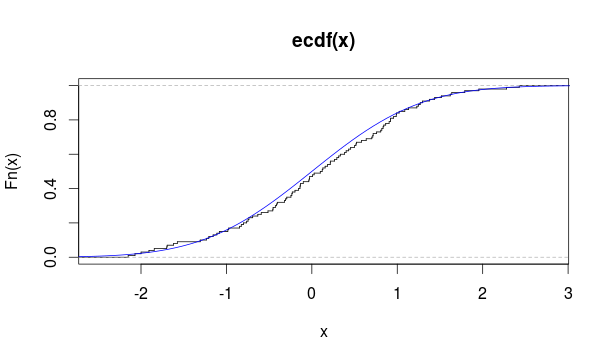
\includegraphics[scale=0.6]{img/KSR.png}
\end{center}*)



ks.test(x,pnorm) # Cierta. Obtenemos un p-valor grande (del orden de 0.7)
ks.test(x,pexp) # Falsa. Obtenemos un p-valor casi 0 (del orden de (*$10^{-16}$*))

\end{lstlisting}


\paragraph{Iteración del contraste} Es bueno repetir el contraste varias veces, ya que la generación de los datos es aleatoria. Para ello,  hay un fichero en moodle de $R$ con el proceso. En las transparencias además, está el otro ejemplo.

\subsection{Gráficos de probabilidad}

Este es otro tipo de contraste. Hemos visto cómo contrastar utilizando \_\_\_ que nos da una $\chi^2$. También hemos utilizado la distribución empírica.

Ahora vamos a ver cómo contrastar utilizando los cuantiles.

Tenemos:
\[
X_1,...,X_n \overset{iid}{\sim} F \implies F(X_n) \overset{iid}{\sim}\mathcal{U}(0,1) \implies F(X_{(i)}) < F(X_{(i+1)})
\]
Podemos calcular:
\[\esp{F(X_{(i)})} = \frac{i}{n+1}\]


Utilizando esta información, podemos dibujar en el eje $x$ de una gráfica los estadísticos de orden $X_{(i)}$ y en el eje $y$, ponemos: $F^{-1}\left(\frac{i}{n+1}\right)$, ya que, en media $F(X_{(i)}) \sim \frac{i}{n+1}$

Lo que esperaríamos si nuestra hipótesis de $F$ fuera cierta, es que los puntos de esa gráfica estén sobre una recta.


\begin{example}
Sea $X_1,...,X_n \overset{iid}{\sim} \underbrace{N(µ,σ^2)}_{F}$. Tomamos $\Phi \sim N(0,1)$


\[X_{(i)} \sim F^{-1}\left(\frac{i}{n+1}\right) = ... = σ\Phi^{-1}\left(\frac{i}{n+1}\right) + µ\]

Si los datos son normales, los puntos $\left( X_{(i)},\Phi^{-1}\left(\frac{i}{n+1}\right)\right)$ estarán alineados.

\end{example}

\obs Este es el tipo de contraste que se utiliza en la realidad para saber si unos datos se distribuyen normalmente o no. Hay una manera de medir esta diferencia y no hacerlo a ojo. Este test se denomina \concept{Shapiro-wilks}




\section{Contrastes de homogeneidad}
\subsection{$\chi^2$ }
Tenemos \[
\left.
\begin{array}{cc}
M_{1} \equiv X_{11} ,...,X_{1n_1} &\overset{iid}{\sim} F_1\\ 
\vdots & \vdots \\
M_{p} \equiv X_{p1} ,...,X_{pn_p} &\overset{iid}{\sim} F_p
\end{array} \right\} H_0 : F_1 = F_2 = ... = F_p 
\]

Con $M_1,...,M_p$, muestras \textbf{independientes}.

\paragraph{Proceso para el contraste}
\begin{enumerate}

\label{contraste::homogeneidad::chicuadrado}

\item Dividimos los datos en clases $A_i$ y consideramos las frecuencias observadas $O_{ij} = \{\#\text{ datos } M_j \text{ en } A_i \}$

\item Al considerar número de $M_j$, tenemos, bajo la hipótesis, que $O_{ij} \equiv B(n_j,p_i)$, con $p_i = P_{H_0}(A_i)$.

\begin{defn}[Tabla de contingencia]
\[
\begin{array}{c|ccc}
&µ_1&\cdots & µ_p \\\hline
A_1 & O_{11} & \cdots & O_{1p}\\
\vdots & \vdots & \ddots & \vdots \\
A_k & O_{k1} & \cdots & O_{kp} 
\end{array}
\]
\end{defn}

\item Las \textbf{frecuencias esperadas} bajo $H_0 \to E_{ij} = n_jp_i$.

\item Construimos el estadístico del contraste. \[\sum_j \sum_i \frac{(O_{ij} - E_{ij})^2}{E_{ij}} \convs[d] \chi^2_{p(k-1)}\]
\subitem \textit{La independencia de las $M_i$ es la que da la convergencia a la $\chi^2$.}

\subitem Dado que no conocemos $p_i$, tenemos que estimarlos a partir de los datos. ¿Cuál es el estimador? Al suponer $F_i = F_j$ podemos utilizar:

\[ \hat{p_i} = \frac{\sum_j O_{ij}}{\sum_j n_j} \implies \hat{E}_{ij} = n_j·p_i = \frac{O_{i·}}{n}O_{·j}\]

\item \textbf{Conclusión} El estadístico es: \[T = \sum_i \sum_j \frac{(O_{ij} - \hat{E}_{ij})^2}{\hat{E}_{ij}} \convs[d] \chi^2_{(p-1)(k-1)} \] 

\subitem ¿Porqué los grados de libertad? Porque al estimar perdemos un grado de libertad por cada estimación, y como aquí estamos estimando $k$ cosas, perderíamos $k$ grados de libertad. El $-1$ aparece porque no hace falta estimar $k$ sino $k-1$ ya que $\sum_i \hat{p_i} = 1$. Entonces $p(k-1) - (k-1) = (p-1)(k-1)$

Y la región de rechazo \[R = \{T>\chi^2_{(k-1)(p-1),α}\}\]

\obs También podemos construir el estadístico como:

\[
T = \sum_{i}\sum_j \frac{O_{ij}^2}{\hat{E_{ij}}} - n
\]

\begin{proof}
Se deja como ejercicio para el lector la afirmación de que el estadístico también se puede construir así.
\end{proof}
\end{enumerate}


\begin{example}

Tenemos 100 observaciones de 3 países (ESP, ITA, FRA) sobre fumadores y queremos saber si las distribuciones que siguen cada tipo de fumador son iguales.

\begin{center}


\begin{tabular}{c|ccc|c}
 & E & I & F & \#\\\hline
NF&30&15&20&65\\
FO&50&40&50&140\\
FH&20&45&30&95\\\hline
&100 & 100 & 100 & 300
\end{tabular}
¿Qué esperamos? $\to$
\begin{tabular}{c|ccc|c}
 & E & I & F & \#\\\hline
NF & 21.6 & 21.6 & 21.6 & 65 \\
FO & 46.6 & 46.6 & 46.6 & 140 \\
FH & 31.6 & 31.6 & 31.6 & 95 \\
\hline
&100 & 100 & 100 & 300
\end{tabular}
\end{center}

Ahora podemos calcular el estadístico y la región de rechazo para $α=0.05$:

\[ T = \sum_{i=1}^k \sum_{j=1}^p \frac{O_{ij}^2}{E_{ij}} -n = ... \sim 16.8\]
\[ c = \chi^2_{4,0.05} = 9.48\]

Como $T > c \implies $ Rechazamos la hipótesis.

\end{example}

\subsection{KS de homogeneidad}

Es importante destacar e este tipo de contraste que sólo es válido para \textbf{dos muestras} y sólo para \textbf{distribuciones continuas}.

Tenemos \[
\left.
\begin{array}{cc}
X_{1} ,...,X_{n} &\overset{iid}{\sim} G\\ 
Y_{1} ,...,Y_m &\overset{iid}{\sim}G
\end{array} \right\} H_0 : F = G
\]

Sean $F_n$ y $G_m$ las funciones de distribución empíricas respectivas.

Calculamos el estadístico de KS para 2 muestras:

\[
D_{n,m} = ||F_n - G_m ||_{\infty} = \sup_{a∈ℝ} | F_n(a) - G_m(a)|
\]
Bajo $H_0$, la distribución de $D_{n,m}$ no depende de $F=G$ y está tabulada (igual que en los contrastes de bondad de ajuste).

Entonces: \[R = \{ D_{n,m} > C_α\}\]
\begin{defn}[Diferencias estandarizadas al cuadrado]
\[
\frac{(O_{ij}-\hat{E_{ij}})}{\sqrt{\hat{E_{ij}}}}
\]
\end{defn} 

\section{Contrastes de independencia}

\subsection{$\chi^2$}

Sean $(X_1,Y_1),...,(X_n,Y_n) \overset{iid}{\sim} F$ con $H_0 : X,Y$ son independientes.

Los datos se suelen dar en tablas por clases, es decir: 

\[
\begin{array}{c|ccc}
&B_1&\cdots & B_p \\\hline
A_1 & O_{11} & \cdots & O_{1p}\\
\vdots & \vdots & \ddots & \vdots \\
A_k & O_{k1} & \cdots & O_{kp} 
\end{array}
\]

Una diferencia con el anterior es que que los totales no están fijados, ya que son variables.

Vamos a ver la estimación de las frecuencias esperadas $\hat{E_{ij}}$ y $E_{ij}$

\begin{align*}
E_{ij} &= n·p_{ij} = n·P(x∈A_i,Y∈B_j) \overset{H_0}{=} n·P(x∈A_i)(Y∈B_j)\\
\hat{E}_{ij} &= n \frac{O_{i·}}{n}\frac{O_{·j}}{n} = \frac{O_{i·}·O_{·j}}{n} \text{ igual que en el anterior}
\end{align*}

Ahora, calculamos $T$ y $R$ exactamente igual que en el contraste de homogeneidad $\chi^2$ \ref{contraste::homogeneidad::chicuadrado}, es decir:

\[T = \sum_i \sum_j \frac{(O_{ij} - \hat{E}_{ij})^2}{\hat{E}_{ij}} \convs[d] \chi^2_{(p-1)(k-1)} \] 

Recordamos que también podemos construir el estadístico como:

\[T = \sum_{i}\sum_j \frac{O_{ij}^2}{\hat{E}_{ij}} - n\]

Y la región de rechazo \[R = \{T>\chi^2_{(k-1)(p-1),α}\}\]


\paragraph{La diferencia entre este contraste y el de homogeneidad} es ...
